\documentclass{article}

\usepackage[ruled,vlined]{algorithm2e}
\usepackage[T1]{fontenc}
\usepackage[utf8]{inputenc}
\usepackage{amsmath}
\usepackage{amsfonts}
\usepackage{amssymb}
\usepackage{amsthm}
\usepackage{authblk}
\usepackage{graphicx}
\usepackage{hyperref}
\usepackage{lmodern}
\usepackage{microtype}
\usepackage{setspace}
\usepackage{subcaption}

\usepackage{graphicx}
\graphicspath{ {img/} }

\usepackage[backend=biber,style=authoryear-comp]{biblatex}
\addbibresource{references.bib}

\title{Generating Synthetic Financial Time-Series Data Through Generative Adversarial Network\\[0.5em] \large Methodologies And Comparison Among Different Deep Learning Structures}

\author[1]{Grant Sawyer\thanks{\href{mailto:gsawyer@andrew.cmu.edu}{gsawyer@andrew.cmu.edu}}}
\author[1]{Harold Yuan\thanks{\href{mailto:zhongfay@andrew.cmu.edu}{zhongfay@andrew.cmu.edu}}}
\author[1]{Kaushik Tallam\thanks{\href{mailto:ktallam@andrew.cmu.edu}{ktallam@andrew.cmu.edu}}}
\author[1]{Mario Nicolo' De Matteis\thanks{\href{mailto:mdematte@andrew.cmu.edu}{mdematte@andrew.cmu.edu}}}
\author[1]{Tristan Roemer\thanks{\href{mailto:troemer@andrew.cmu.edu}{troemer@andrew.cmu.edu}}}

\affil[1]{Carnegie Mellon University, MSCF, New York, USA}

\usepackage{cleveref}
\usepackage{geometry}
\geometry{a4paper, margin=1in}

\date{February 2025}

\begin{document}

\maketitle

\begin{abstract}
    Generative Adversarial Networks (GANs) have emerged as a powerful tool for synthesizing realistic financial time series data by addressing challenges such as data scarcity, privacy, and cost. This paper explores the integration of attention mechanisms, convolutional neural networks (CNNs), and long short-term memory (LSTM) layers within a GAN framework to generate synthetic financial price data. We evaluate the performance of these architectures using three financial instruments: JPMorgan Chase (JPM), Apple Inc. (AAPL), and the MSCI ACWI Index (ACWI). The data spans over two decades of market data. Our results demonstrate that CNN enhanced GANs significantly improve the modeling of temporal dependencies and volatility clustering compared to Attention and LSTM based variants. The synthetic data exhibits statistical properties that align with real world financial time series which is validated by tests for distributional similarity and moments. These findings provide actionable insights for financial institutions seeking to augment datasets for backtesting, risk management, and machine learning applications.
\end{abstract}

\doublespacing

\noindent \textbf{Keywords:} Generative Adversatial Networks, Financial Time-Series, Attention Layers

\section{Introduction}

Hedge Funds, Proprietary Trading Firms, and other financial institutions rely on large amounts of data to make informed decisions. However, obtaining high-quality financial data can be challenging due to privacy concerns, data access restrictions, and the high cost of data acquisition. To address these challenges, researchers have developed generative models that can synthesize realistic financial time-series data. These models can be used to augment existing datasets, generate new data for backtesting trading strategies, and simulate market conditions for risk management. Over the last few years, many different developments have been conducted in the field of synthethic financial time-series data generation. In this paper, we provide a comprehensive overview of the methodologies and comparison among different deep learning structures used to generate synthetic financial time-series data. In particular, we aim to synthesize new price time series data that can be highly useful for various applications. These include backtesting trading strategies, training machine learning models, and conducting stress tests and scenario analyses. By generating realistic synthetic data, we can provide financial institutions with a valuable resource to enhance their decision-making processes, improve model robustness, and better prepare for adverse market conditions.

Given the great impact and power of generative AI models, we decided to exploit one of the main pillars of Generative AI: the Generative Adversarial Network develope by \textcite{goodfellow_generative_2014}. GANs have been extensively used in the computer vision field, particularly in image generation. \textcite{iglesias_survey_2023} show the ability to generate realistic data samples through adversarial training makes them a powerful tool for synthesizing financial time-series data as well. This groundbreaking model has profoundly influenced subsequent research by demonstrating that adversarial training can generate remarkably realistic data samples. \textcite{EckerliFlorian2021GANi} mentions different applications of GANs, including market manipulation, credit card fraud, portfolio optimization and market prediction.

In the realm of synthetic financial data, several other aspects are equally important. For example, robust data augmentation techniques can enhance model reliability, and careful evaluation of synthetic data against real-world financial indicators is crucial for ensuring its practical utility. Moreover, addressing the temporal dependencies and non-linear dynamics inherent in financial markets requires advanced modeling techniques that go beyond the original GAN framework. In simple terms, we aim to find out the distribution by which the prices have been generated. When looking for new data, among the most well-known techniques, we recall different and exotic sampling techniques that tend to be very complex and computationally expensive. As highlighted by \textcite{cont_empirical_2001}, understanding the empirical properties of asset returns, such as heavy tails and volatility clustering, is essential for developing realistic financial models. These properties must be carefully considered when designing synthetic data generation frameworks to ensure that the generated data accurately reflects the behavior observed in real financial markets.

We designed the neural networks for the GAN models by implementing three different types of layers: Attention, CNN, and LSTM. We decided to implement these three different types of layers because each offers unique advantages for capturing the complex dynamics of financial time series data. In accordance with the literature, Attention layers allow the model to focus on significant temporal patterns, enhancing its ability to prioritize key segments of the data. Convolutional Neural Networks (CNNs) are effective at detecting localized patterns and extracting spatial features, which are crucial for modeling short-term trends and volatility clusters. Long Short-Term Memory (LSTM) networks excel at capturing long-range dependencies and the sequential nature of financial data, making them ideal for modeling the temporal evolution of asset prices. By integrating these diverse neural network components, we aim to improve the overall performance and robustness of our GAN models in generating realistic synthetic financial time series data.

Building on these insights, our paper aims to explore and compare the effectiveness of various neural network architectures within the GAN framework. In particular, we focus on:
\begin{itemize}
    \item \textbf{Attention Layers}: To capture and prioritize significant temporal patterns, thereby enabling the model to focus on key segments of the time series.
    \item \textbf{Convolutional Neural Networks (CNNs)}: To detect localized patterns and extract spatial features from financial time series data.
    \item \textbf{Long Short-Term Memory (LSTM) Networks}: To model long-range dependencies and effectively capture the sequential characteristics of financial data.
\end{itemize}

Through a detailed comparative analysis, this study evaluates the performance of these architectures in generating synthetic financial time series data. In particular, we investigate how the integration of attention mechanisms can enhance the synthesis process by more accurately reflecting the intricate dynamics of financial markets.

\vspace{1em}
\noindent\textit{The project code, datasets, and additional resources are available at our GitHub repository: \url{https://github.com/mariodematteis/ml-ii-final-project}.}

\section{Data and Variables of Interest}

The purpose of this paper is to generate synthetic time series data from a Generative Adversarial Network (GAN) framework. To that end, it is important to carefully consider what financial instruments to use for training and testing the model so that it is both robust and easily generalized. The three instruments that we chose to analyze in this paper are JPMorgan Chase (JPM), Apple Inc. (AAPL), and the MSCI ACWI Index (ACWI). We specifically chose these equity securities because they allow us to assess the performance of our model across both individual equities and a broad market index, which when put together, helps us represent a wide array of market dynamics.

We sourced the time series data that was used in this paper from the Wharton Research Data Services (WRDS) platform, which provided access to very high quality daily historical data. We extracted data from January 1, 2000 to January 31, 2024 for tickers JPM and APPL. We chose a large time frame in order to cover multiple market cycles and include significant past economic events, which should potentially allow the model to capture the complex dynamics that are inherent in the financial markets over time. For example, the model will be able to see both periods of high volatility, like the 2008 financial crisis and the 2020 Covid-19 pandemic, as well as the periods of relative stability in between.

For the MSCI ACWI index, we decided to extract data from the iShares MSCI ACWI ETF which tracks the overall performance of the MSCI ACWI index. However, since this fund was created in 2008, we were only able to extract data from March 28, 2008 to January 31, 2024. Even though we have less time series data for the index compared to the individual stock data, because the index represents a well diversified portfolio of global equities, in both emerging and developed markets, the context it provides is important for evaluating the generalizability of the synthetic data that our model generates across different market conditions and geographic regions.

By using these datasets, we can comprehensively evaluate our GAN based approach. In the following sections, we will describe the preprocessing steps that were applied to the raw data, including cleaning, normalization, and the transformation procedures, that were used to make the data more suitable for model training.

\section{Model}

Generative Adversarial Networks (GANs) provide a framework to learn complex data distributions through a two-player minimax game involving two neural networks: a \textbf{generator} and a \textbf{discriminator}. The classical formulation of GANs is outlined below, after which we describe our enhanced generator architectures that incorporate attention, convolutional, and long short-term memory layers.

\subsection*{1. Setup and Notation}

\begin{itemize}
    \item \textbf{Real Data Distribution:} Let $p_{\text{data}}(x)$ denote the probability distribution of real data samples $x \in \mathcal{X}$.
    \item \textbf{Latent Space and Prior:} Define a latent space $\mathcal{Z}$ with a simple prior distribution $p_z(z)$ (e.g., a Gaussian or uniform distribution). A latent variable $z \sim p_z(z)$ is sampled and then transformed into the data space.
    \item \textbf{Generator:} The generator is a function $G: \mathcal{Z} \to \mathcal{X}$ parameterized by $\theta_G$. It maps a latent variable $z$ to a synthetic sample $G(z)$, thereby inducing an implicit distribution $p_g(x)$ over the data space.
    \item \textbf{Discriminator:} The discriminator is a function $D: \mathcal{X} \to [0,1]$ parameterized by $\theta_D$. It outputs a scalar representing the probability that a given sample $x$ originates from the real data distribution $p_{\text{data}}(x)$ rather than from $p_g(x)$.
\end{itemize}

\subsection*{2. The Minimax Game}

The GAN framework is formulated as a two-player minimax game with the value function

\[
\min_{G} \max_{D} V(D,G) = \mathbb{E}_{x\sim p_{\text{data}}(x)}\big[\log D(x)\big] + \mathbb{E}_{z\sim p_z(z)}\big[\log (1 - D(G(z)))\big].
\]

\begin{itemize}
    \item \textbf{Discriminator’s Objective:} For a fixed generator $G$, the discriminator $D$ is trained to maximize the probability of correctly classifying real data and generated data:

    \[
    \mathbb{E}_{x\sim p_{\text{data}}(x)}\big[\log D(x)\big] + \mathbb{E}_{x\sim p_g(x)}\big[\log (1 - D(x))\big].
    \]

    \item \textbf{Generator’s Objective:} Simultaneously, the generator $G$ is trained to minimize the same objective (i.e., to “fool” $D$) by generating samples $G(z)$ that maximize the discriminator's misclassification:

    \[
    \min_{G} \mathbb{E}_{z\sim p_z(z)}\big[\log (1 - D(G(z)))\big].
    \]
\end{itemize}

\subsection*{3. Optimal Discriminator and Jensen-Shannon Divergence}

For any fixed generator $G$, the optimal discriminator $D^*_G(x)$ is obtained by maximizing the value function pointwise:
\[
f(D(x)) = p_{\text{data}}(x) \log D(x) + p_g(x) \log (1 - D(x)).
\]
Taking the derivative with respect to $D(x)$ and setting it to zero leads to:
\[
\frac{p_{\text{data}}(x)}{D(x)} - \frac{p_g(x)}{1-D(x)} = 0 \quad \Longrightarrow \quad D^*_G(x) = \frac{p_{\text{data}}(x)}{p_{\text{data}}(x) + p_g(x)}.
\]
Substituting $D^*_G$ back into the value function yields:
\[
V(G, D^*_G) = -\log(4) + 2\, \mathrm{JSD}\big(p_{\text{data}} \,\|\, p_g\big),
\]
where $\mathrm{JSD}$ denotes the Jensen-Shannon Divergence. Minimizing $V(G, D^*_G)$ with respect to $G$ forces $p_g(x)$ to converge to $p_{\text{data}}(x)$.

\subsection*{4. Training Procedure}

In practice, GAN training alternates between:
\begin{enumerate}
    \item \textbf{Discriminator Update:} Maximize $V(D, G)$ with respect to $\theta_D$, keeping $\theta_G$ fixed.
    \item \textbf{Generator Update:} Minimize $V(D, G)$ (or a modified loss, such as maximizing $\log D(G(z))$ for stronger gradients) with respect to $\theta_G$, while keeping $\theta_D$ fixed.
\end{enumerate}
These updates are typically performed using stochastic gradient descent or its variants. In our specific case, for each of the model trained we used the Adam optimizer with a learning rate of $ 0.0002 $ for both the Discriminator and the Generator.

\subsection*{5. Enhanced Generator Architectures}

While the classical GAN framework provides a robust foundation for generative modeling, financial time series data pose unique challenges due to their complex temporal dependencies and nonlinear structures. To address these issues, we extend the generator architecture by incorporating advanced neural network components, as detailed below.

\subsubsection*{5.1 Attention Layers}

Attention mechanisms have revolutionized various fields, particularly natural language processing, by allowing models to dynamically focus on different parts of the input sequence \textcite{vaswani_attention_2023}. In our generator, we incorporate a Self-Attention layer inspired by this work. The attention mechanism computes a weighted sum of feature representations across time steps, enabling the model to prioritize significant temporal patterns. This approach is particularly beneficial for capturing long-range dependencies and subtle patterns in financial data. In quantitative finance, attention-based models have garnered significant interest; for example, \textcite{qin_dual-stage_2017} introduced a dual-stage attention-based recurrent neural network for time series prediction, while \textcite{chen_exploring_2019} leveraged attention mechanisms for enhanced stock price forecasting. Our implementation integrates a series of deconvolutional layers followed by a Self-Attention module, thereby enhancing the model's capability to generate realistic and coherent time series data.

\subsubsection*{5.2 Convolutional Neural Networks (CNNs)}

CNNs are well-suited for detecting localized patterns and extracting spatial features from time series data. By applying convolutional filters along the temporal dimension, CNNs can capture short-term trends and volatility clusters, which are crucial for modeling the non-stationary characteristics of financial markets. Our generator architecture includes deconvolutional layers that progressively upsample the latent representation, allowing the model to generate detailed and realistic time series data. The effectiveness of CNNs in time series forecasting and anomaly detection has been demonstrated in various studies, including \textcite{lecun_deep_2015}. Moreover, a growing body of literature has shown that CNNs excel in quantitative finance applications. For instance, \textcite{dixon_high_2017} illustrated their utility in market trend forecasting, while \textcite{liu_option_2023} and \textcite{zhang_deeplob_2019} demonstrated their capabilities in option pricing, risk management, volatility prediction, and anomaly detection in high-frequency trading data. These studies underscore the versatility and robustness of CNN architectures in capturing complex, localized patterns within financial datasets.

\subsubsection*{5.3 Long Short-Term Memory (LSTM) Networks}

LSTM networks are designed to capture long-term dependencies in sequential data, making them ideal for modeling the temporal evolution of financial time series. The gating mechanisms in LSTMs allow the network to retain relevant information over extended periods, addressing issues such as vanishing gradients. Our LSTM-based generator includes fully connected layers to transform the latent space into a suitable input for the LSTM layers, followed by an output layer that generates the final time series. The use of LSTMs in financial modeling has been extensively studied, as highlighted by \textcite{hochreiter_long_1997}.

While LSTMs have historically been a cornerstone in Natural Language Processing (NLP) for tasks such as language modeling and machine translation (\textcite{sutskever_sequence_2014, fischer_deep_2018}), the emergence of attention-based mechanisms—introduced by \textcite{bahdanau_neural_2016} and further advanced by \textcite{vaswani_attention_2023}—has largely supplanted them in that field. In contrast, within quantitative finance, LSTMs remain a robust tool. Their ability to model sequential dependencies has proven valuable in a range of applications, including market trend forecasting (\textcite{fischer_deep_2018}), risk management (\textcite{bao_deep_2017}), and volatility prediction, where capturing temporal nuances is critical.

\subsubsection*{5.4 Integration within the GAN Framework}

In our proposed model, these enhanced architectural components are integrated within the generator network while the discriminator maintains a conventional architecture. The overall training procedure remains consistent with the classical GAN framework, with the generator updates now encompassing additional hyperparameters related to the attention heads, convolutional filter sizes, and LSTM layer configurations.

The evaluation provides insights into how these components improve the generator's ability to model the intricate, nonlinear, and temporal structures present in real financial time series.


\section{Results and Evaluations}

As can be seen in the appendix, the CNN implementation performs better than the other two models. Visually, the log returns of the generated data look very similar to the log returns of the historical data. We can note, however, the model does not adequately capture the market dynamics for JP Morgan. The results tend to not be very aligned with the true observed distribution of returns for this stock.

Analyzing the results from a more statitical perspective, like the Jensen-Shannon divergence, the model based on the convolutional layers shows best results. Again, Apple and the MSCI ACWI Index yield better results than JPM. Looking at the Jensen-Shannon Divergence for CNN (JSD, min. of 0 and max. of $ ln(2) = 0.693 $) we get a score in the order of $ 10^{-1} $ which is very good. JPM on the otherhand is quite high with a score of 0.251.

The generated distribution for JPM has considerably fatter tails, especially a fatter left tail which would explain why all the generated time series plotted for JPM have a drastic negative spike in one concentrated area. This may have been caused by a large drawdown during a short time period in the historical data that the model overemphasized during training, or perhaps a data error. The LSTM model performs worst according to JSD and produces too narrow of a distribution. This may indicate that there was some sort of structural mistake in applying that architecture to our data. Perhaps, after tuning the architecture more appropriately for our data and retraining, we would achieve better results. The attention model manages to produce better distributions than the LSTM, however, the distributions are also not strongly aligned with historical data. Specifically for ACWI, the Attention architecture does quite okay (visually) with a JSD of 0.222. Overall, both visually and numerically, the CNN GAN strongly outperforms the other architectures used.

It is also interesting to look at autocorrelation for our time series which is another important metric of market dynamics. In our historical data, JPM and ACWI showed evidence of autocorrelation, while AAPL did not. This can be seen in the Ljung-Box tests in the tables in the appendix. Our generated data showed autocorrelation for all 3 tickers in all 3 models. This means that it either correctly generates autocorrelated data for 2/3 tickers, or, the architecture and methodology potentially always generates autocorrelated data.

\section{Conclusion}

In conclusion, our investigation into enhanced GAN architectures for synthesizing financial time series data demonstrates that incorporating convolutional layers yields superior performance in capturing the distributional characteristics of asset returns compared to LSTM and attention based models. While the CNN based model successfully replicates the historical return distributions for instruments such as AAPL and the MSCI ACWI Index, discrepancies observed for JPM highlight areas for further refinement. More work should be done to explore additional tuning of the architectures and to consider hybrid approaches that combine the strengths of attention, CNNs, and LSTMs to achieve even closer alignment with observed market data. These improvements could provide financial institutions with robust synthetic datasets for applications in backtesting, risk management, and machine learning research.

\section*{Acknowledgments}

We would like to thank CodeWilling for providing the computational resources that enabled us to train and evaluate our models effectively.

\printbibliography

\appendix
\section{Appendix}

\begin{table}[ht]
\centering
\begin{tabular}{lcc}
\hline
\textbf{Metric} & \textbf{Original} & \textbf{Generated} \\
\hline
Mean     & 0.000128 & -0.000002 \\
Std      & 0.040645 & 0.214407 \\
Skewness & -25.111799 & 0.255764 \\
Kurtosis & 1039.042700 & 46.728140 \\
Ljung-Box t-statistic & 10.673040 & 272346.309774 \\
Ljung-Box p-value & 0.383552 & 0.000000 \\
\hline
\end{tabular}
\caption{AAPL Moments Comparison for the Attention-Based GAN.
Jensen--Shannon Divergence: 0.580034}
\label{tab:aapl_attention}
\end{table}

\begin{table}[ht]
\centering
\begin{tabular}{lcc}
\hline
\textbf{Metric} & \textbf{Original} & \textbf{Generated} \\
\hline
Mean     & 0.000279 & 0.000001 \\
Std      & 0.012906 & 0.079548 \\
Skewness & -0.556542 & -0.786310 \\
Kurtosis & 11.866263 & 135.567522 \\
Ljung-Box t-statistic & 55.307795 & 1234.989861 \\
Ljung-Box p-value & 0.000000 & 0.000000 \\
\hline
\end{tabular}
\caption{ACWI Moments Comparison for the Attention-Based GAN.
Jensen--Shannon Divergence: 0.221720}
\label{tab:acwi_attention}
\end{table}

\begin{table}[ht]
\centering
\begin{tabular}{lcc}
\hline
\textbf{Metric} & \textbf{Original} & \textbf{Generated} \\
\hline
Mean     & 0.000189 & -0.000002 \\
Std      & 0.104471 & 0.198215 \\
Skewness & -0.021890 & 0.098549 \\
Kurtosis & 106.470019 & 30.823050 \\
Ljung-Box t-statistic & 1442.181508 & 247959.786055 \\
Ljung-Box p-value & 0.000000 & 0.000000 \\
\hline
\end{tabular}
\caption{JPM Moments Comparison for the Attention-Based GAN.
Jensen--Shannon Divergence: 0.504067}
\label{tab:jpm_attention}
\end{table}

\begin{table}[h!]
\centering
\begin{tabular}{lcc}
\hline
\textbf{Metric} & \textbf{Original} & \textbf{Generated} \\
\hline
Mean     & 0.000128 & 0.000003 \\
Std      & 0.040645 & 0.180111 \\
Skewness & -25.111799 & -0.640448 \\
Kurtosis & 1039.042700 & 158.044933 \\
Ljung-Box t-statistic & 10.673040 & 347.086390 \\
Ljung-Box p-value & 0.383552 & 0.000000 \\
\hline
\end{tabular}
\caption{AAPL Moments Comparison for the CNN-Based GAN.
Jensen--Shannon Divergence: 0.060796}
\label{tab:aapl_cnn}
\end{table}

\begin{table}[h!]
\centering
\begin{tabular}{lcc}
\hline
\textbf{Metric} & \textbf{Original} & \textbf{Generated} \\
\hline
Mean     & 0.000279 & -0.000001 \\
Std      & 0.012906 & 0.082028 \\
Skewness & -0.556542 & -0.880490 \\
Kurtosis & 11.866263 & 143.158931 \\
Ljung-Box t-statistic & 55.307795 & 264.902105 \\
Ljung-Box p-value & 0.000000 & 0.000000 \\
\hline
\end{tabular}
\caption{ACWI Moments Comparison for the CNN-Based GAN.
Jensen--Shannon Divergence: 0.065261}
\label{tab:acwi_cnn}
\end{table}

\begin{table}[h!]
\centering
\begin{tabular}{lcc}
\hline
\textbf{Metric} & \textbf{Original} & \textbf{Generated} \\
\hline
Mean     & 0.000189 & -0.000001 \\
Std      & 0.104471 & 0.174060 \\
Skewness & -0.021890 & 1.247102 \\
Kurtosis & 106.470019 & 60.163179 \\
Ljung-Box t-statistic & 1442.181508 & 64169.776953 \\
Ljung-Box p-value & 0.000000 & 0.000000 \\
\hline
\end{tabular}
\caption{JPM Moments Comparison for the CNN-Based GAN.
Jensen--Shannon Divergence: 0.251107}
\label{tab:jpm_cnn}
\end{table}

\begin{table}[h!]
\centering
\begin{tabular}{lcc}
\hline
\textbf{Metric} & \textbf{Original} & \textbf{Generated} \\
\hline
Mean     & 0.000128 & -0.000005 \\
Std      & 0.040645 & 0.168739 \\
Skewness & -25.111799 & 0.647168 \\
Kurtosis & 1039.042700 & 150.256361 \\
Ljung-Box t-statistic & 10.673040 & 1412.511109 \\
Ljung-Box p-value & 0.383552 & 0.000000 \\
\hline
\end{tabular}
\caption{AAPL Moments Comparison for the LSTM-Based GAN.
Jensen--Shannon Divergence: 0.608428}
\label{tab:aapl_attention}
\end{table}

\begin{table}[h!]
\centering
\begin{tabular}{lcc}
\hline
\textbf{Metric} & \textbf{Original} & \textbf{Generated} \\
\hline
Mean     & 0.000279 & -0.000000 \\
Std      & 0.012906 & 0.084201 \\
Skewness & -0.556542 & 2.924553 \\
Kurtosis & 11.866263 & 80.666600 \\
Ljung-Box t-statistic & 55.307795 & 3032.228573 \\
Ljung-Box p-value & 0.000000 & 0.000000 \\
\hline
\end{tabular}
\caption{ACWI Moments Comparison for the LSTM-Based GAN.
Jensen--Shannon Divergence: 0.601836}
\label{tab:acwi_lstm}
\end{table}

\begin{table}[h!]
\centering
\begin{tabular}{lcc}
\hline
\textbf{Metric} & \textbf{Original} & \textbf{Generated} \\
\hline
Mean     & 0.000189 & 0.000002 \\
Std      & 0.104471 & 0.120360 \\
Skewness & -0.021890 & -0.977749 \\
Kurtosis & 106.470019 & 132.980503 \\
Ljung-Box t-statistic & 1442.181508 & 6376.462484 \\
Ljung-Box p-value & 0.000000 & 0.000000 \\
\hline
\end{tabular}
\caption{JPM Moments Comparison for the LSTM-Based GAN.
Jensen--Shannon Divergence: 0.596089}
\label{tab:jpm_lstm}
\end{table}

\begin{figure}[h!]
    \centering
    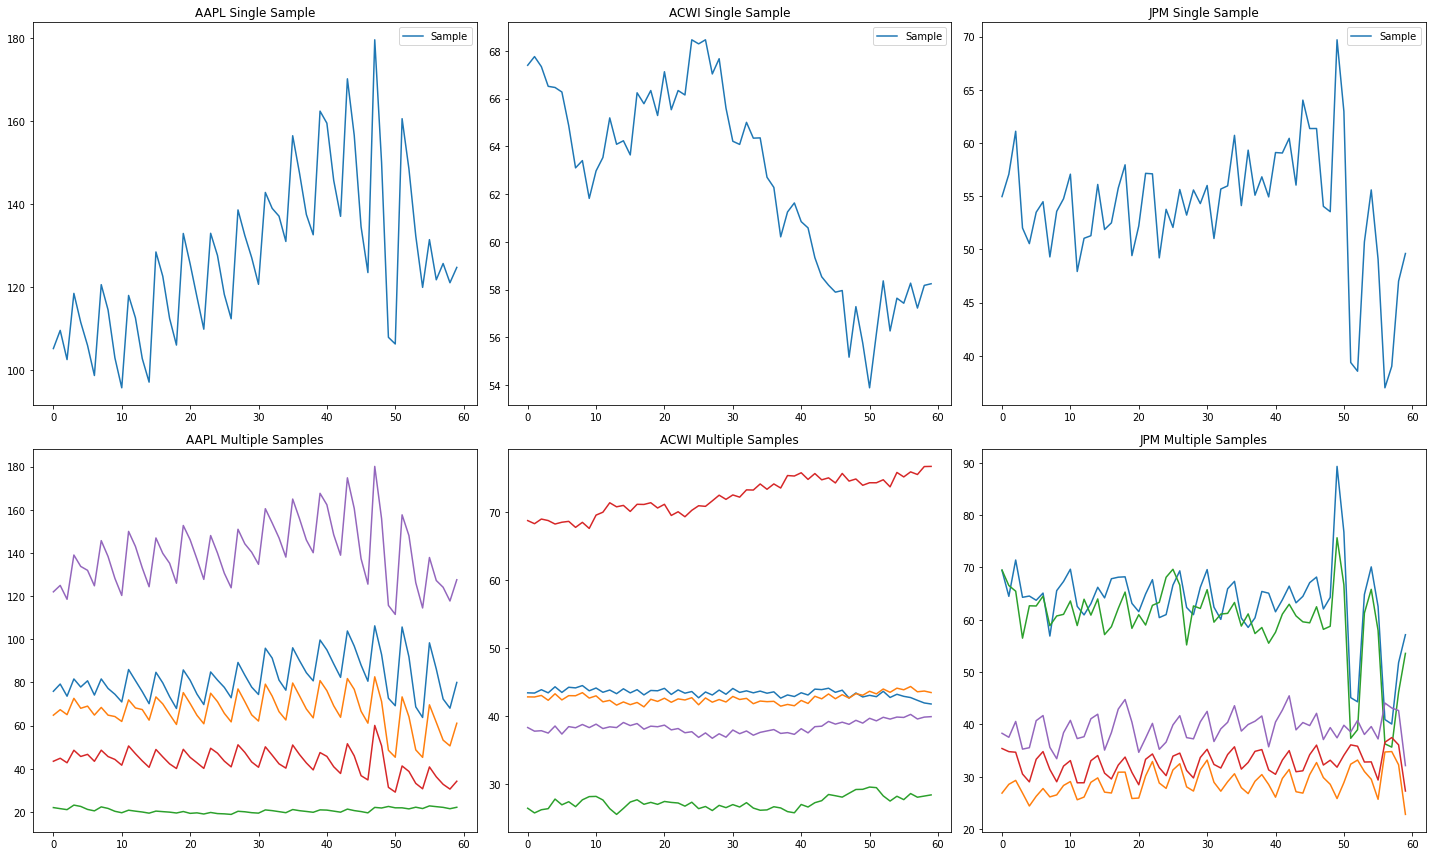
\includegraphics[width=0.7\textwidth]{attention_gen_samples}
    \caption{Comparison of Real vs. Generated Time Series for AAPL, ACWI and JPM using Attention-Based GAN.}
    \label{fig:attention_comparison}
\end{figure}

\begin{figure}[h!]
    \centering
    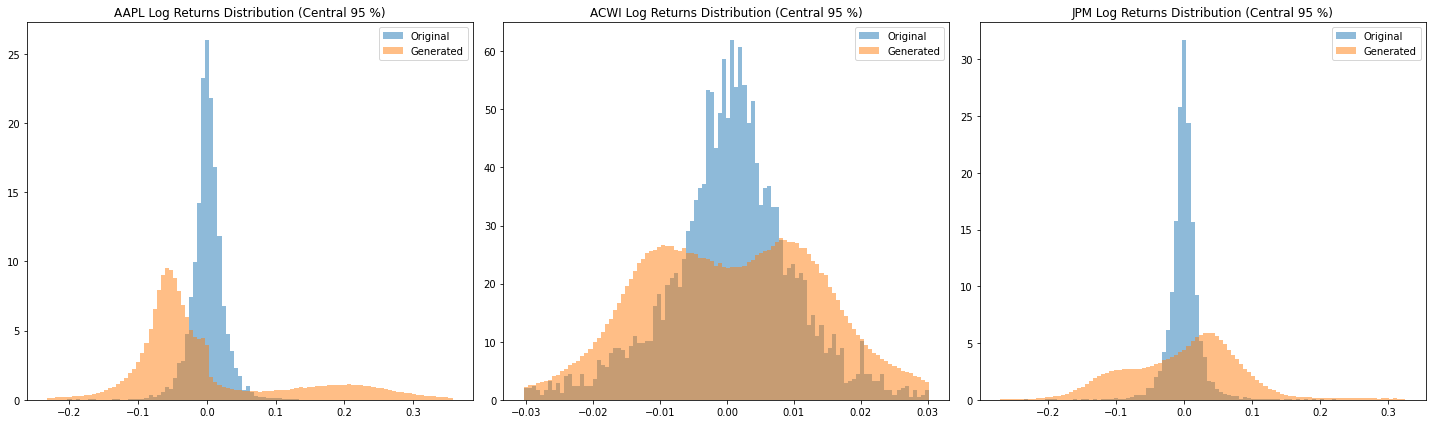
\includegraphics[width=0.7\textwidth]{attention_distributions}
    \caption{Comparison of Real vs. Generated Log-Return Distributions for AAPL, ACWI and JPM using Attention-Based GAN.}
    \label{fig:attention_comparison}
\end{figure}

\begin{figure}[h!]
    \centering
    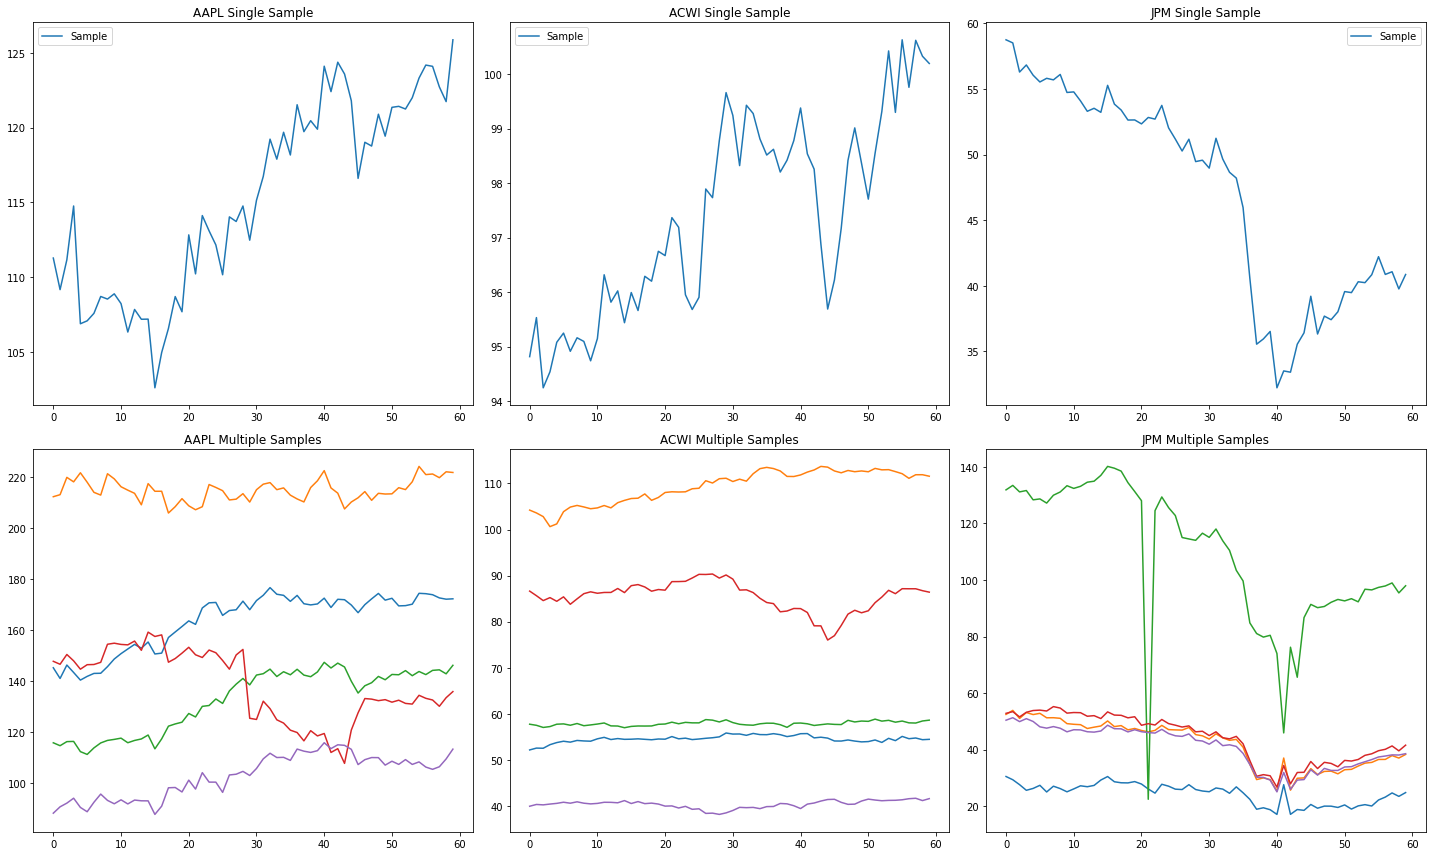
\includegraphics[width=0.7\textwidth]{CNN_gen_samples}
    \caption{Comparison of Real vs. Generated Time Series for AAPL, ACWI and JPM using Attention-Based GAN.}
    \label{fig:attention_comparison}
\end{figure}

\begin{figure}[h!]
    \centering
    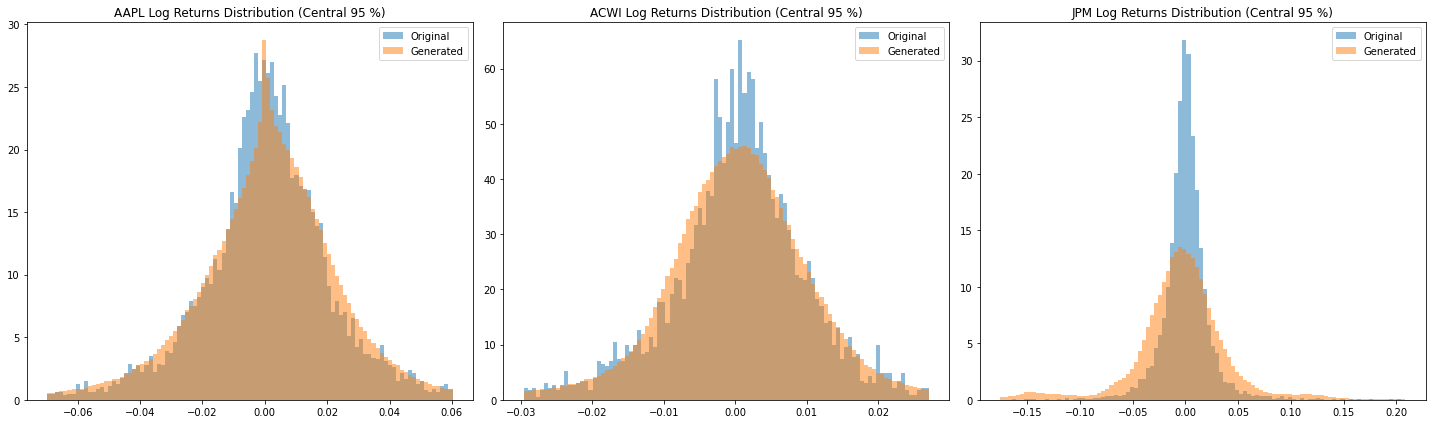
\includegraphics[width=0.7\textwidth]{cnn_distributions}
    \caption{Comparison of Real vs. Generated Log-Return Distributions for AAPL, ACWI and JPM using CNN-Based GAN.}
    \label{fig:attention_comparison}
\end{figure}

\begin{figure}[h!]
    \centering
    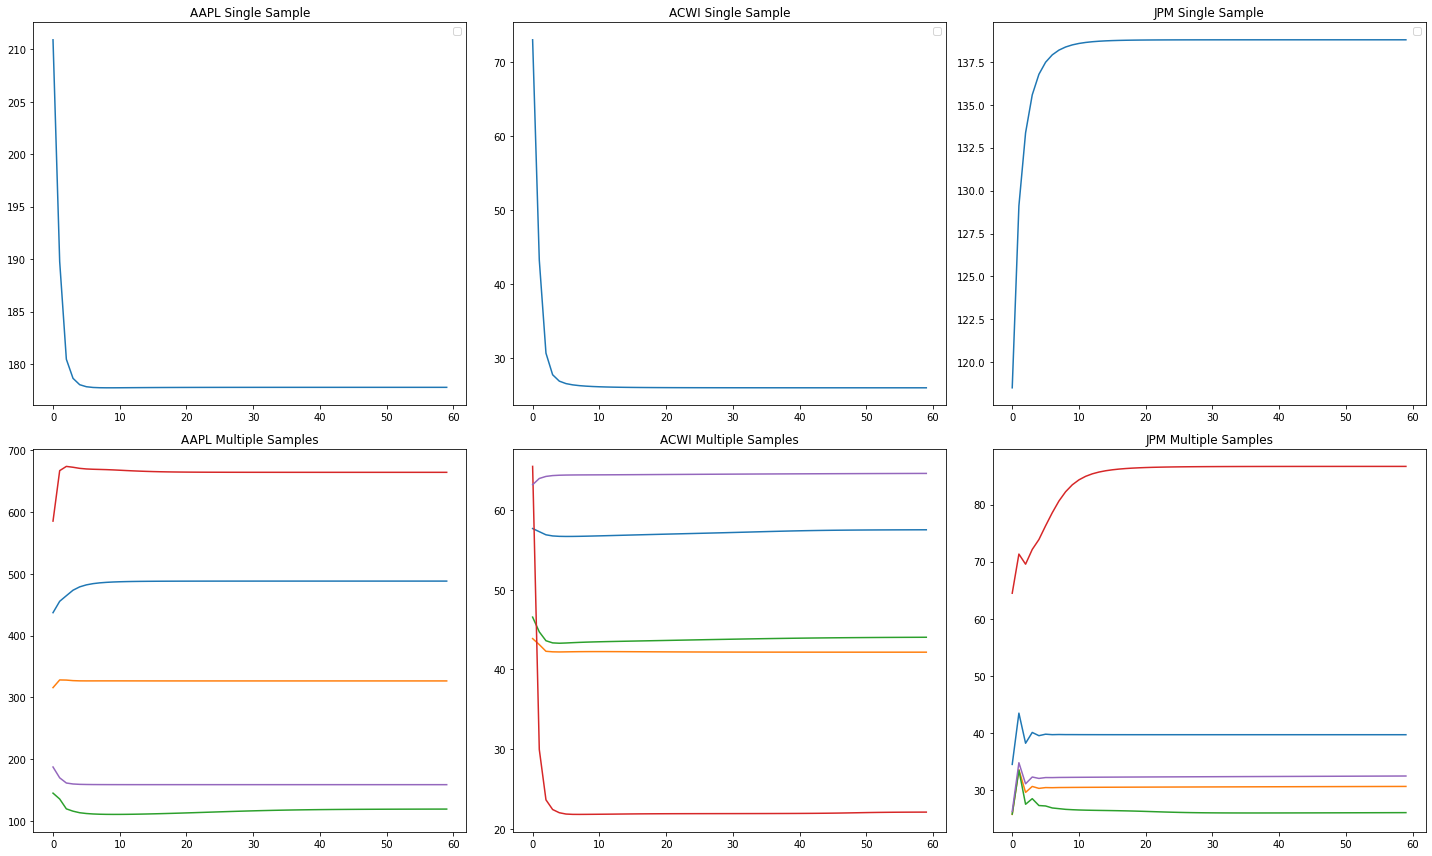
\includegraphics[width=0.7\textwidth]{LSTM_gen_samples}
    \caption{Comparison of Real vs. Generated Time Series for AAPL, ACWI and JPM using LSTM-Based GAN.}
    \label{fig:attention_comparison}
\end{figure}

\begin{figure}[h!]
    \centering
    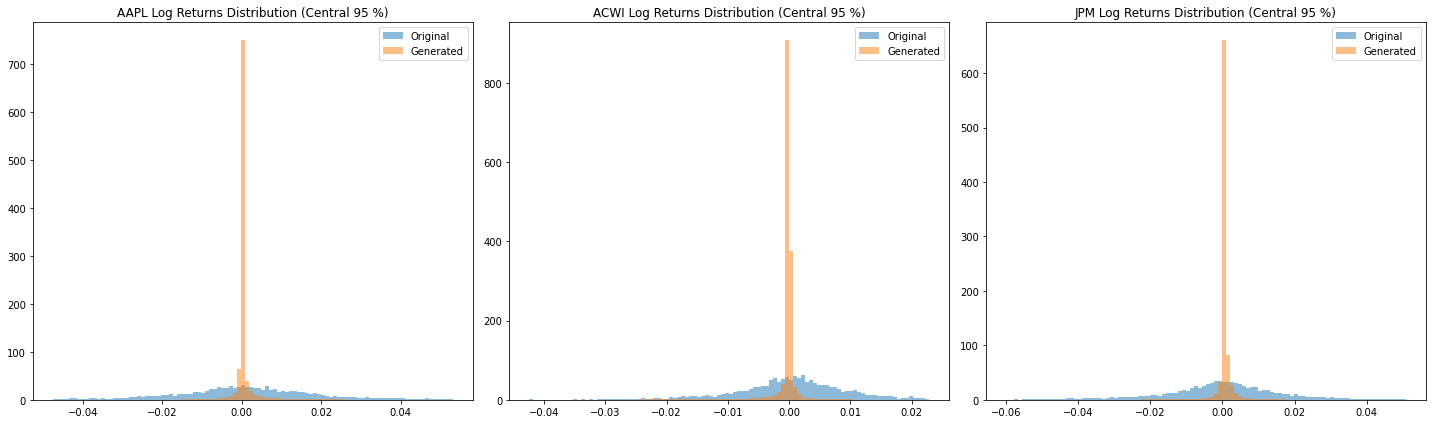
\includegraphics[width=0.7\textwidth]{LSTM_distributions}
    \caption{Comparison of Real vs. Generated Log-Return Distributions for AAPL, ACWI and JPM using LSTM-Based GAN.}
    \label{fig:attention_comparison}
\end{figure}

\end{document}
